\documentclass{article}
\usepackage{graphicx}
\begin{document}

% --- TITLE PAGE --- %

\begin{titlepage}
\newcommand{\HRule}{\rule{\linewidth}{0.5mm}}
\center
\textsc{\LARGE Imperial College London}  \\[1.5cm]
\textsc{\Large Department of Computing}  \\[0.5cm]
\textsc{\large Course 350: Management and Business for Computing Engineers} \\[0.5cm]

\HRule \\[0.6cm]
{\huge \bfseries SubZero Ice} \\[0.3cm]
\HRule \\[1.5cm]

\begin{minipage}{0.4\textwidth}

% author
\begin{flushleft} \large \emph{Authors:} \\
Tim       \textsc{Gates}   \\
Ben       \textsc{Homer}   \\
Graham    \textsc{Lyon}    \\
Conor     \textsc{Nevin}   \\
Martin    \textsc{Sidery}  \\
Jon       \textsc{Watson}  \\
\end{flushleft}

% lecturer
\end{minipage}~
\begin{minipage}{0.4\textwidth}

\begin{flushright} \large \emph{Lecturer:} \\
Nick \textsc{Coutts}
\end{flushright}

\end{minipage}\\[2cm]

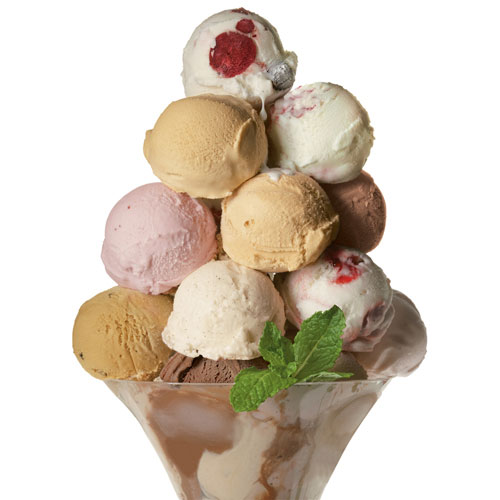
\includegraphics[scale=0.3]{ice_cream.jpg}

\end{titlepage}

\pagebreak

\tableofcontents

\pagebreak

%Disclaimer page

%TODO: Add table here see original example template

\section{Disclaimer}
This business plan has been prepared by SubZero Ice and is being provided to a limited number of persons, at their request.  This document is confidential and is only being made available to parties who agree to keep it confidential.  Neither this business plan nor any part of it shall be copied, reproduced or distributed to others at any time without the prior written consent of SubZero Ice. By accepting this document the recipient is deemed to undertake and warrant to SubZero Ice that the recipient will keep it confidential and that the recipient shall return all copies of this document to SubZero Ice immediately upon request.
Although SubZero Ice has taken reasonable care to ensure that the information contained in this document is accurate, no other representation or warranty, express or implied, is or will be given by SubZero Ice or any of its agents.  No responsibility is or will be accepted by SubZero Ice or any of its agents as to the accuracy or completeness of this document or the information or opinions contained herein.  Recipients must make their own investigations and must satisfy themselves as to the condition and prospects of SubZero Ice and the accuracy and completeness of statements contained herein.
Any financial projections given in this plan are illustrative only.  Because of the early stage nature of SubZero Ice’s business, none of the projections given in this document should be taken as guaranteed to be attainable, nor should they be taken as implying any indication, assurance or guarantee that those assumptions are correct or exhaustive.

%TODO: Add table here see original example template
\pagebreak

\tableofcontents

\pagebreak

%-------------------------------------------------------------------------------

\section{Executive summary}

SubZero Ice is an innovative business aimed at providing ice-cream in a more personal, novel and exciting way. Our patented process allows us to use liquid-nitrogen as a freezing agent, providing customers with delicious, velvety smooth ice-cream along with a fantastic visual display as they watch their chosen ice-cream being prepared. What sets us apart from the competition is our focus on providing a unique customer experience as well as producing the highest quality ice-cream. In addition our instantly recognisable laboratory-themed stalls and enthusiastic ice-cream makers ensure that no one can pass us by unnoticed. We also pride ourselves on our use of fresh, organic ingredients in all of our products. \\

At the current time our main business focus is on acquiring a positive reputation at prestigious public events throughout the UK. During this period of growth and learning our business has recieved a remarkable amount of interest from some of the major event organisers in the UK as well as some press coverage. We have recieved hundreds of invitations to operate our stalls at public events, however given the relative age of our business coupled with our rapid success, we currently do not have to capital required in order to meet the demands of our expanding customer base. Having seen firsthand how customers react to our product we believe that it is time to take our relatively small business to the next level, hopefully expanding the area within which we operate to the whole of the UK. \\

Some of the companies that have already shown an interest in our business include the London Science Museum, Alton Towers, Odeon Cinemas, London Royal Parks and the organisers of music and arts festivals such as Glastonbury, Reading and Latitude. We have provided ice-cream and entertainment with much success at a large variety of events and demonstrations across England.


\section{Vision statement}

Our main goal is and always will be not only to provide great tasting ice-cream for our customers but also to provide them with an memorable experience. We strongly believe that their is a direct relationship between the amount of fun our staff are having and the number of customers we can attract. We also place the highest priority on producing quality ice-cream as we realise that even if the novelty of our product begins to fade over time, we will still be making the tastiest ice-cream on the market. \\

SubZero Ice is a worker cooperative meaning that all of our staff can have a say on any decisions which need to be made. This structure has helped us to create a workforce who intrinsically care about the business and its future. We place great importance on being both ethical and economical within all spheres of business. All our stalls use solar panels to generate energy and our staff all follow a strict recycling policy which helps us to reduce costs as well as doing our bit for the environment. The majority of our fresh ingredients are fairtrade and organic as we believe that in order to make the best ice-cream we need to use the best ingredients. Additionally our customers can choose how healthy or luxurious they would like their ice-crean to be by customising their choice of indgredients. We also provide comprehensive training for all our staff to ensure that they can safely handle liquid nitrogen. \\

Assuming that we manage to raise enough capital to expand our business activites over the next few years, we plan to focus our attention on scaling up our resources to match our ever increasing customer demand. At the same time we hope to branch out in other directions by introducing new products and also streamlining our specialised equipment which will allow our products to be introduced to establishments in the hospitality sector such as at bars and cafes.

\section{Market Analysis}
  
  Before delving into our business structure and our ideas for the future we though it would be wise to give a general overview of the current state of the ice-cream and conveniene foods markets so that the reader can gain a deeper insight into the current climate we are working in.

  \subsection{Market Drivers and Trends}

   We first take a look at current trends within the markets we are involved with and relate each observation to our own business. We hope that by predicting the direction the market will take we will be able to meet and exceed our customer's expectations.

   - The ice-cream market boasted a 9\% value growth in 2012, an improvement over the increase seen in 2011. It is believed that this increase is mainly due to good product innovation, large marketing campaigns and a renewed desire to purchase indulgance foods in the UK. We therefore feel that now would be a great time to expand our business to take advantage of this period of value growth in the market.

   - It has been noted by several market experts that people do not seem to be holding back on purchasing culinary treats even during times of economic challenge. The ice-cream market has even seen growth during some of the hardest periods for the UK economy. It has been suggested that people are seeking comfort foods more often as a result of increased stress, leading to overall market growth.

 - The use of liquid nitrogen in consumer food products is increasing as more businesses turn to \"molecular gastronomy\" (the science of investigating and explaining how physical and chemical transformations can be made during cooking) in order to improve the taste and visual appeal of thier products. For example, some modern chefs use liquid nitrogen in the kitchen to change the consitancy of food. The cocktail industry have already taken note of this trend and have started to introduce products which use liquid nitrogen, mainly for its visual effect. We predict that in the future more companies will turn to molecular gastronomy in order to gain a competitive advantage. Since we have patented our unique ice-cream making process, which makes use of liquid nitrogen, we feel that we are in a strong position to take the majority market share for our niche in the market. 

 - Events and hospitality companies are constantly looking to put on more of a show to gain an advantage over competitors and attract more people. Large festivals such as the main music festivals are attracting more people each year. We therefore intend to make it a priority to have stalls at these events as they will give us a lot of public exposure. We currently have a strong relationship with some of the major event mangers in the UK and we hope to solidify our partnership with them even more in the future.

 - Historically successful ice-cream products are primarily those which have the most market appeal and capture the consumers imagination. With our product we hope to generate lots of consumer interest through our unique approach to ice-cream. However, in order to retain our customers our ice-cream must also taste
better than our competitors. We believe our fresh ingredients and luxuriously smooth ice-cream will ensure that this is the case. It is generally accepted that innovation will be the main driver of growth over the next few years, with many ice-cream companies focussing on developing new products, particularly in the premium segment, as indulgence remains a key consumer trend. We believe that our product will be able to satisfy this desire for innovation and quality seen at the current time, while also being more affordable than most of the premium brands on the market.

- The London Olymipics has had a large impact on the ice-cream market with sales expected to top the £1bn mark for the first time in 2013.

- In comparison the the ice-cream market, the frozen yoghurt market is relativaly underdeveloped and is therefore an area of opportunity. At SubZero Ice we have already begun researching how we can use our patented process to produce frozen yoghurts in the future.


  \subsection{Market Segments}

  The ice-cream products currently on sale can be segmented as the diagram below shows.
  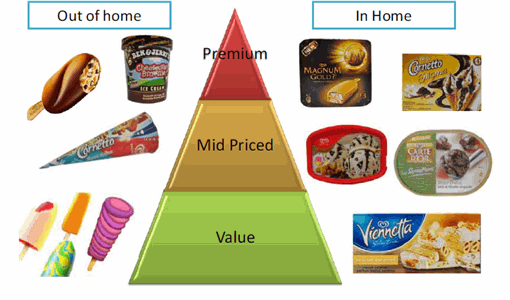
\includegraphics[scale=0.3]{pricepyramid.gif}

  Value ice-cream brands

  Premium brands - becoming increasingly popular in the UK.

  Convenience brands - ice-creams which are meant to be eaten outside

  Mostly prepackaged - very few ice-cream producers sell their products directly to customers but rather through retailers.

  We intend to do things differently from the majority of the market, by making ice-cream which not only tastes better than that of our competitors but is also delivered to the customer in a more exciting and personal way.


  \subsection{The Opportunity for SubZero Ice}
  Introduction to the market...

   - We are at the forefront of developing market having already established ourselves as an exciting and innovative new brand.

    and want to grow this market through the hospitality industry.

 - We believe that we provide a better, more scalable product than competitors and are therefore in prime position to take the majority of the market share.

   - With current technology must target venue hire

   - Interest expressed by other firms eg: Odeon

  Target market - tourists, guests and families at large events of all varieties & developing prepackaged products which we can sell via retailers

  Market Context

  Market size \& characteristics - very few ice-cream vendors who sell from stalls

  Market Validation


\section{Products and Services We Offer}
  Detail of what we are actually going to offer

  Current products - ice-cream & frozen yoghurt (very underdeveloped market - chance to change this)
    -- fresh ingredients, keep use of preservatives to a minimum

  Stall/Staff overview

  Future products



\section{Business Model \& Structure}
  How the business will actually work

Workers cooperative mode

Suits set up of company (started by group of friends)

Means every stall holder/operator is interested in business development

Currently have sold … and have established technology

Currently have capability to operate … stalls

Currently marketing via word of mouth as well as ringing venues.
Hoping to establish long term customers.

Distribution model ??????

Supply chain??

  \subsection{Longterm \& Shorterm Goals}

    objective - maximise sales -> how

     % summary of detailed plan including
	% prioritisation
	% validation
	% offers
	% routes to market

  \subsection{Current Equity Structure}

  \subsection{Management team}

Jon Watson has many years experience working with and managing small
businesses. He prides himself on the fact that every small business which he has managed has gone on to be highly successful. His attention to detail and vast experience working with start-ups make him an invaluable leader and we feel privileged that he has chosen to work with us. He is considered an expert in discovering what makes a small businesses tick and in finding ways to develop a unique culture within a business.


\section{Competition}

  Unilever UK Ltd is currently the leading business in the ice-cream market, with a 30\% market share in 2012. The company's retail sales saw a 22\% increase during the same year, indicating the level of growth the market is currently going through. Unilevers most popular brands are Magnum and Cornetto. They are also the global business operators of Ben & Jerry's, Cart D'Or and Walls. The company continues to offer new varients on existing products which have all been well recieved by the public. Recently they have also been spending large amounts on advertising which has also increased their success. For example the release of Ben & Jerry's Core range was supported by a huge £5 million advertising campaign.

  R&R Ice Cream are the other notable market leader, owning brands such as Nestle, Ribena, Kelly's of Cornwall and Thorntons.  
  Small number of direct competitors

  Certainly none with the success and interest that we have already generated

  In terms of mainstream ice-cream companies...


  \subsection{Competitive Advantage}

We believe our product has several clear competitive advantages over
other ice-cream brands currently on the market. Below we list some of these advantages.

 - Our ice-cream is velvety smooth, creamy and freshly made. Due to
the unique freezing process our ice-cream is guaranteed to be free of
large ice crystals giving a delicious texture like no other ice-cream on the
market.

 - Our process instantly freezes the freshest of ingredients, providing
an unsurpassed flavour. Since we make the ice-creams freshly for
our customers it means there is also much more scope for different
flavourings. Customers can choose any of our fresh ingredients they like and combine them in any way they choose.

 - Another clear competitive advantage of using liquid nitrogen is that
it provides a unique and fascinating spectacle that normal ice cream
stalls simply cannot provide. We believe that creating an impressive
visual experience for our customers and putting on a show is almost
as important as the ice-cream itself. Through this unique blend
of entertainment and delicious ice-cream we hope to capture the
imaginations of our customers.

 - We also have the advantage of novelty. Many consumers will never
have tried or even heard of liquid nitrogen ice-cream before and so
we hope that one-off novelty purchases will help us to be even more
successful, especially during the first few years of business.

 - Since the customer has complete control over the ingredients which are used in their ice-cream, apart from the base ingredients, our ice-creams have the potential to be more healthy than our competitors. This can only help, given the current trend towards healthy, low-fat foods.

\section{Intellectual Property Assets}

  \subsection{Patents}
    Patented process

In terms of technology we currently use standard liquid nitrogen storage tanks at our stalls. Our innovation is not in the technology we use but in how we use it. All of our equipment is carefully designed to fit in with our stores' laboratory theme. We also use smoke machines and coloured smoke to make our stalls look more visually appealing.

We hope to raise enough capital to be able to purchase more compact storage units, in order to branch out our business into cafe's or bars.

  \subsection{Know-How}

  \subsection{Future Intellectual Property Development}

  Want to shrink product for use in bars

  Development already started

\section{Business Development Plan}

  \subsection{Current Structure \& Resources}

  \subsection{Sales process}

  \subsection{Target customers}
Tourists of all ages. Especially families with children and young adults
who are more likely to be at festivals.

 - Want to move away from small temporary stalls to more permanent
installations

 - Want to target large customers in the hospitality sector

 - Odeon, Alton Towers, Thorpe Park?

   LTV = (Tn + ATV + LT) - (CoA + CoR)
       = (no + average transaction value + lifetime value) - (cost of aquisition + cost of retention) 

  \subsection{Current key customers}

  Currently provided product as one off temporary stall for 

  They have expressed interest in returning to us

  \subsection{Marketing, PR and Communications}
  At the moment our main form of marketing are the stalls themselves.
Given the exciting way we present our product the stalls often generate
a lot interest, which large groups of people watching our ice-cream
being made simply out of interest before they make a purchase.

In the future as we move into more permanent fixtures we hope to use
more traditional marketing methods.???

We are currently developing a website which we think will play a vital
role in generating more consumer interest. Through this website we will
give our customers the opportunity to contact us and leave feedback on
their experience with our product.

We also wish to focus strongly on interacting with social media sites
such as Facebook and Twitter as we believe this will allow us to quickly
generate interest, receive comments and interact directly with our
customers. Additionally this will allow us to collect information about
our customers, for example the average age of our customers. It is with
such information that we hope to be able to tailor our future marketing.

In order to generate interest online we will hold regular competitions
and prize draws, in which the winners will receive vouchers to spend on
our ice-cream. We also plan to video some of our stalls in action and
post on YouTube.???

  \subsection{Staff Recuritment}

  Currently all of our staff operate from our headquarters in central London. As our customer base expands we will need to recruit the following staff:

 \bold{Ice-cream Makers} – ice-cream makers are the life and soul of SubZero Ice. In order to qualify for the role candidates will have to show genuine enthusiasm and commitment to the company as well as being able to work well under pressure infront of crowds. Candidates must also be very flexible as they will have to travel to different locations each day if not working at a fixed stall. All ice-cream makers will receive suitable training and must pass a health and safety test to ensure they can safely handle liquid nitrogen and that they understand the risks of using liquid nitrogen on a daily basis. Perks include free entry to large festivals, free ice-cream and the opportunity to have fun at work.

 \bold{Marketing and PR Staff} - our marketing staff have the huge responsibility of creating relationships with potential clients (event managers) and generating public interest in our unique brand and products. They have the opportunity to shape our future and maximise our success. In order too qualify candidates must have a flair for marketing, be able to listen to the ideas of others and give constructive feedback. Some members of the PR staff will also be responsible for managing our online prescence by replying to customers, making note of customer feedback and creating competitions and prize-draws for customers.

\bold{Product Designers} - our product designers must realise what our customers want before they want it. In order to qualify for this role candidates must have worked with at least one previous product design team and be able to think laterally. Product designers work with our current brand and public image to create new and exciting products. At SubZero Ice we are not scared of change and so we also encourage our product designers to be innovative by having weekly meetings in which adventourous theories or experimental product ideas can be discussed and shared.

\bold{Transport Team} – our transport team are responsible for moving our stalls and equipment to events and setting them up. They are also responsible for taking all equipment back to our nearest storage hold after it has been used. All candidates must have a full UK driving license and will be given relevant health and safety training on starting. Members of the transport team must be flexible as they will have different working hours depending on which events we are currently operating at. They may also have to transport our equipment from one storage depot to another when we require more equipment in a certain area of the country.

 \bold{Finance Team} - our finance team are responsible for assessing our current finances, analysing what could be done better and producing financial projections. All canditates must have a strong mathematical background and the desire to make a positive difference to our company. As a business we do not want to rely on gut feelings as to what is optimal for our business but on real world data and mathematical models. Our finance team are therefore responsible for deciding how we should balance our spending as a company in order to increase our profit and the overall value of SubZero Ice.

 \bold{Legal Team} - we will require a small team of specialised legal associates who can advise us on legal matters especially as our business grows and we receive more clients. Although members of the legal team will technically be external to the company, they will all be granted membership of the business cooperative and hence will be able to buy and sell shares within the company.


  \subsection{Facilities}

  We already own a small office in central London from which we operate.
  Will need large office as number of staff increases.

  Currently store equipment in a storage warehouse when not in use.
  Will need new storage locations around the country to make access to equipment easier.


\section{Funding \& Financial Plan}
Add more subsections

We are looking to raise £5 million in captial, to allow us to expand our business and develop our range of products.

Main costs:
 - Stalls - LN2 tanks + supply - 50 litre liquid nitrogen tanks – around £1000 & Each litre of liquid nitrogen costs around £1.25
 - Transport vechicles
 - Storage space
 - Staff recruitment and wages
 - New London HQ - expand existing offices - £0.5 million
 - Ice cream ingredients
 - Marketing and website




Each litre of ice-cream requires...

Office and storage space in London will cost

Ideally we would like the capital to be able to purchase equipment to
produce our own liquid nitrogen from the air.(???)

Use of Funds

More stalls

More marketing needed

Need to grow beyond London

Professional website and web prescence on social media sites


SHARES

Revenue from sales in the previous year was around £3.5 million. (total income without subtracting any expenses) 
Gross profit of £2.9 million (difference between sales and cost of sales i.e. revenue - cost of goods)
Net profit of £1.8 million (actual profit when all expenses are subtracted)

%Graph to show financial growth over first year of business


revenue
 - retail
   licence
   other sales

profit/net income
 - gross
   net
   EBITDA
   NPV

costs
 ...

\section{Risk Analysis \& Exit Strategy}



\section{Corportate Information \& Contact Details}

\end{document}
